\documentclass{beamer}
\usetheme{simple}
\usepackage[brazil]{babel}
\usepackage[utf8]{inputenc}
\usepackage{lmodern}
\usepackage[scale=2]{ccicons}

\usepackage{graphicx,hyperref,url,pgfplots}
\usepackage{amsmath} 
\usepackage{array,booktabs}
\pgfplotsset{compat=1.15} 

\setbeamercovered{invisible}
\newcommand{\pausar}{\pause}
\newcommand{\df}[1]{\,\mathrm{d}#1}
\newcommand{\parcial}[3]{\dfrac{\partial^{#1}#2}{\partial #3^{#1}}}

\title{Cinemática e Dinâmica}
\subtitle{Equações de Movimento}
\date{\today}
\author{Jeferson Lima}
\institute{\url{http://gitlab.com/jeferson.lima}}

\begin{document}

\maketitle

\begin{frame}{Informações Úteis}
	\begin{block}{Material disponível em:}
		\href{Robótica Móvel - Wiki}{https://gitlab.com/cursoseaulas/robotica-movel/-/wikis/home}
	\end{block}
	\pausar
	\begin{block}{Datas Importantes}
		\begin{itemize}
		\item Entrega
		\item Envio
		\end{itemize}
	\end{block}
	\pausar
	\begin{block}{Requisitos da Disciplina}
		\begin{itemize}
		\item Teoria de Controle
		\item Linguagem de Programação - \textbf{Python} ou \textbf{C++}
		\item Eletrônica
		\end{itemize}
	\end{block}
\end{frame}

\begin{frame}{Descrição de Posição e Orientação}
\begin{center}
    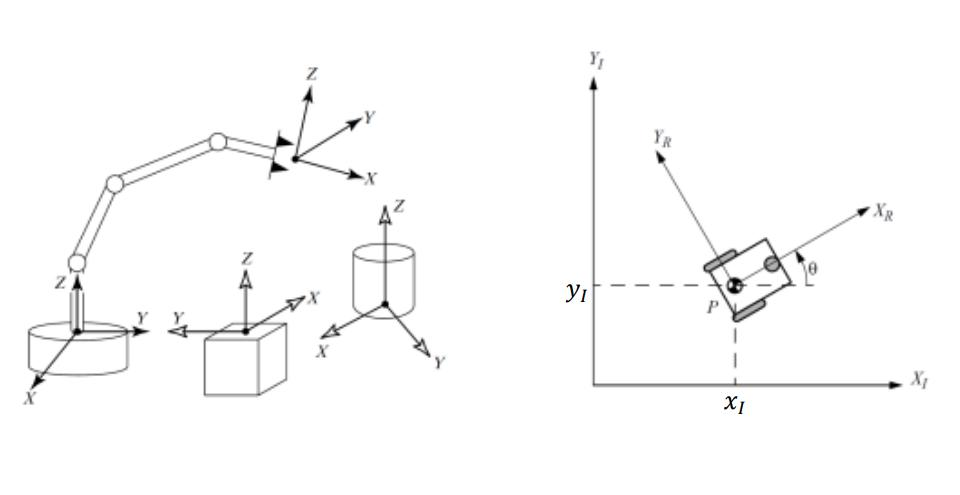
\includegraphics[width=0.8\textwidth]{images/mecanismos.jpg}
\end{center}
\end{frame}


\begin{frame}{Descrição de Posição e Orientação}
    \begin{itemize}
		\item coordenada como um vetor de posição $\mathbb{R}^{3 \times 1}$, composto pelas coordenadas $X,Y$ e $Z$.
		\item um ponto ${}^A\mathbf{P}$ representa a distância ao longo dos eixos do plano $\{A\}$. Os elementos individuais de ${}^A\mathbf{P}$ podem ser visto pela equação \eqref{eq:cine1}.
	\end{itemize}
	\begin{columns}[c]
			\begin{column}{0.6\textwidth}
			\begin{figure}
				\centering
				\begin{tikzpicture}[scale=0.8]
				\node(p0) at (0,0){};
				\draw [->] (p0.center) --++(0,3) node[right] {$ Y_A$};
				\draw [->, rotate =120] (p0.center) --++(0,3) node[below] {$ Z_A$};
				\draw [->, rotate =240] (p0.center) --++(0,3) node[below] {$ X_A$};
				\draw [->] (p0.center) --++(2.5,0.5) node(B)[above,rotate=30] {${}^A\mathbf{P}$};
				\node at (-1.5,2.5) {$\{A\}$};
				\end{tikzpicture}
				\caption{Vetor em relação ao plano $\{A\}$}
				\label{fig:cine1f}
				\end{figure}
		\end{column}
		\begin{column}{0.3\textwidth}
			\begin{equation}\label{eq:cine1}
				{}^A\mathbf{P} = \begin{bmatrix}
				p_x\\ p_y \\ p_z
				\end{bmatrix}
				\end{equation}			
		\end{column}
	\end{columns}
\end{frame}



\begin{frame}{{Translação Rotação e Transformação}}
  \framesubtitle{Matriz de Rotação}
  \begin{itemize}
    \item O vetor definido por ${}^A\mathbf{P}$ pode ser rotacionado pela matriz de rotação $\mathbf{R}$, conforme a equação \eqref{eq:cine2}.
    \begin{equation}\label{eq:cine2}
        {}_A^B
        \mathbf{R} = 
        \begin{bmatrix}
        r_{11} & r_{11} & r_{11}\\
        r_{21} & r_{21} & r_{21}\\
        r_{31} & r_{31} & r_{31}\\
        \end{bmatrix}
        \end{equation}
\end{itemize}

\begin{block}{Considera os exemplos}
    \begin{equation*}
        \mathbf{R}(\theta) = 
        \begin{bmatrix}
            \cos \theta &-\sin \theta \\\sin \theta &\cos \theta
        \end{bmatrix}
        \end{equation*}
    ou:
    \begin{equation*}
        \mathbf{R}_z(\theta) = 
        \begin{bmatrix}
        \cos(\theta) & \sin(\theta) & 0\\
        \sin(\theta) & \cos(\theta) & 0\\
        0 & 0 & 1\\ 
        \end{bmatrix} \text{, eixo $Z$ fixo}
        \end{equation*}
\end{block}

\end{frame}





\begin{frame}{{Translação Rotação e Transformação}}
    \framesubtitle{Matriz de Rotação}
    \begin{block}{}
        \begin{equation*}
            \mathbf{R}_x(\theta) = 
            \begin{bmatrix}
            1 & 0 & 0\\
            0 & \cos(\theta) & -\sin(\theta)\\
            0 & \sin(\theta) & \cos(\theta)\\ 
            \end{bmatrix} \text{, eixo $x$ fixo}
        \end{equation*}
        \begin{equation*}
            \mathbf{R}_y(\theta) = 
            \begin{bmatrix}
            \cos(\theta) & 0 & \sin(\theta) \\
            0 & 1 & 0\\
            -\sin(\theta)  & 0 & \cos(\theta)\\ 
            \end{bmatrix} \text{, eixo $y$ fixo}
        \end{equation*}
        \begin{equation*}
            \mathbf{R}_z(\theta) = 
            \begin{bmatrix}
            \cos(\theta) & \sin(\theta) & 0\\
            \sin(\theta) & \cos(\theta) & 0\\
            0 & 0 & 1\\ 
            \end{bmatrix} \text{, eixo $z$ fixo}
        \end{equation*}
    \end{block}
  
  \end{frame}


\begin{frame}{{Translação Rotação e Transformação}}
    \framesubtitle{Rotação de um coordenada}
    \begin{itemize}
        \item A rotação, em torno e $Z $, de um angulo qualquer $\theta$ em ${}^AP$ é descrita como na equação \eqref{eq:cine3}. 
        \begin{equation}\label{eq:cine3}
            {}^B\mathbf{P} = {}_A^B \mathbf{R}(\theta) {}^A\mathbf{P} = 
            \begin{bmatrix}
            \cos(\theta) & \sin(\theta) & 0 & 0\\
            \sin(\theta) & \cos(\theta) & 0 & 0\\
            0 & 0 & 1 & 0\\ 
            0 & 0 & 0 & 1\\
            \end{bmatrix}.
            \begin{bmatrix}
            {}^Ap_x\\
            {}^Ap_y\\
            {}^Ap_z\\
            1
            \end{bmatrix}
            \end{equation}
    \end{itemize}
\end{frame}


\begin{frame}{{Translação Rotação e Transformação}}
    \framesubtitle{Translação}
    \begin{itemize}
        \item O Deslocamento é chamado de translação, e dá-se pelo operador translacional $\mathbf{D}_A(q)$, onde ${}^A\mathbf{Q}$ representa uma translação entre os planos $\{A\}$ e $\{B\}$ e é expresso pela equação \eqref{eq:cine4}.
        \begin{equation}\label{eq:cine4}
        {}^A\mathbf{Q} =
        \begin{bmatrix}
        q_x\\ q_y \\ q_z
        \end{bmatrix}, \qquad \mathrm{e} \qquad
        \mathbf{D}_A = 
        \begin{bmatrix}
        1 & 0 & 0 & q_x\\
        0 & 1 & 0 & q_y\\
        0 & 0 & 1 & q_z\\
        0 & 0 & 0 & 1
        \end{bmatrix}.
        \end{equation}
    \item Adota-se agora a notação para translação e rotação de um vetor, conforme a equação \eqref{eq:cine5}. Observa-se que a matriz $\mathbf{D}_A$ foi incorporada pela nova notação.
        \begin{equation}\label{eq:cine5}
        \begin{bmatrix}
        {}^B_A\mathbf{P}\\ 1
        \end{bmatrix}
        =
        \underbrace {
        \left[
        \begin{matrix}
        & {}_B^A\mathbf{R}& \\ \hline
        0 & 0 & 0\\
        \end{matrix} \right.
        \left.
        \vline
        \begin{matrix}
        {}^A\mathbf{Q}\\ \hline
        1
        \end{matrix} \right]
        }_{{}^A_B\mathcal{A}}
        \begin{bmatrix}
        {}^B\mathbf{P}\\
        1
        \end{bmatrix}
        \end{equation}
    \end{itemize}
\end{frame}


\begin{frame}{{Translação Rotação e Transformação}}
    \framesubtitle{Operação de Translação e Rotação}
    \begin{itemize}
        \item Aplicando se a transformação homogênea da coordenada ${}^AP$ pelos operadores de rotação e translação temos ${}^BP$
        \begin{figure}[!ht]
        \centering
        \begin{tikzpicture}[scale=0.7]
        \node(p0) at (0,0){};
        \draw [->] (p0.center) --++(0,3) node[right] {$\hat Y_A$};
        \draw [->, rotate =120] (p0.center) --++(0,3) node[below] {$\hat Z_A$};
        \draw [->, rotate =240] (p0.center) --++(0,3) node[below] {$\hat X_A$};
        \draw [->, dotted] (p0.center) --++(1.5,4) node(B)[above,rotate=30] {${}^A\mathbf{P}$ ou ${}^A\mathbf{P}_{BORG}$};
        \node(p1) at (6,1){};
        \draw [->, rotate =30] (p1.center) --++(0,3) node[right,rotate=30] {$\hat Y_B$};
        \draw [->, rotate =150] (p1.center) --++(0,3) node[below,rotate=30] {$\hat Z_B$};
        \draw [->, rotate =270] (p1.center) --++(0,3) node[below,rotate=30] {$\hat X_B$};
        \draw [->] (p1.center) --++(1.5,4) node(B)[above,rotate=30] {${}^B\mathbf{P}$};
        \draw [dotted,-latex] (p0)  -- (p1) node[midway, fill=white]{${}^A\mathbf{Q}$};
        \draw [-latex,dashed] (p0)  -- (B);
        \node at (-1.5,2.5) {$\{A\}$};
        \node at (4,2.5)  [rotate=30]   {$\{B\}$};
        \end{tikzpicture}
        \label{fig:cine2}
        \end{figure}
    \end{itemize}
\end{frame}

\begin{frame}{{Translação Rotação e Transformação}}
    \framesubtitle{Transformação Homogênea}
    \begin{itemize}
        \item Na forma generalizada, a transformação homogênea ${}^{i}_0\mathbf{T}$ pode ser expressa por uma sucessiva pode ser encontrada fazendo o produto das sucessivas transformações de ${}^{i-1}_0\mathcal{A}_i$. Conforme é mostrado na equação \eqref{fig:cine3}.
        \begin{equation}\label{fig:cine3}
        \begin{array}{lcl}
        {}^i_0\mathbf{T} &= & {}^0_1\mathcal{A}{}^1_2\mathcal{A} \cdots {}^{i-1}_i\mathcal{A} = \prod \limits^i_{j=1}{}^{j-1}_i\mathcal{A}, \quad \mathrm{para\;}i=1,2,\cdots,n\\[.2cm]
        & = &
        \begin{bmatrix}
        x_i & y_i & z_i & p_i\\
        0 & 0 & 0 & 1
        \end{bmatrix} = 
        \begin{bmatrix}
        {}^i_0\mathbf{R} & {}^i_0\mathbf{P}\\
        \mathbf{0} & 1
        \end{bmatrix}
        \end{array}
        \end{equation}      
        \item onde, ${}^i_0\mathbf{P}$ é o vetor de orientação do referencial $i$ em relação a base $0$.
    \end{itemize}

\end{frame}

\begin{frame}{{Translação Rotação e Transformação}}
\framesubtitle{Exemplo Numérico}

\end{frame}

\begin{frame}{Exercicios}
    \begin{enumerate}
        \item A
        \item B
    \end{enumerate}
\end{frame}


\begin{frame}{{Cinemática}}
    \framesubtitle{}
    \begin{itemize}
        \item A equação de cinemática  \ref{ex:cinematica}, temos:

        \begin{equation}
        \mathcal{T} = \sum\limits_{i=0}^{N} \frac{1}{2} m {}_{i}^{i+1} \dot{\mathbf{P}}^T \cdot {}_{i}^{i+1}\dot{\mathbf{P}}+ J\boldmath{\omega}_i^T\cdot \boldmath{\omega}_i,
        \end{equation}
    \end{itemize}
\end{frame}



\begin{frame}{{Dinâmica}}
    \framesubtitle{}

    \begin{equation}
        \mathcal{L}= \mathcal{T} - \mathcal{V}
    \end{equation}
    
    \begin{equation}\label{eq:hamiles3}
        \frac{d}{\df{t}}\left( \parcial{}{\mathcal{L}}{\dot{q}_i}\right) - \frac{d \mathcal{L}}{d q_i} + \parcial{}{R}{\dot{q}_i}= 0, \quad i = 1,2,...,n
        \end{equation}
        
\end{frame}



\begin{frame}[c]{{Modelagem de um Uniciclo}}
    \framesubtitle{}
    \centering
    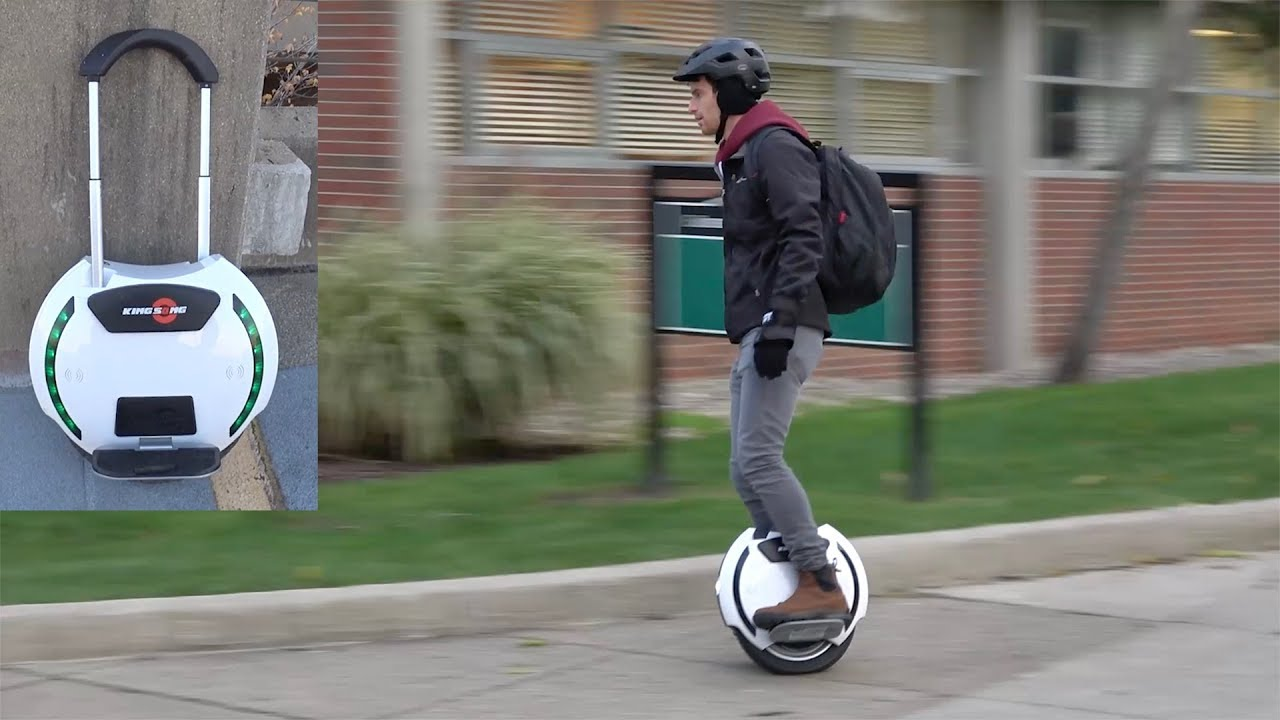
\includegraphics[width=0.8\textwidth]{images/unicycle.jpg}
\end{frame}



\begin{frame}[c]{{Modelagem de um Uniciclo}}
    \framesubtitle{}
    \begin{columns}
        \begin{column}[c]{0.4\textwidth}
            \centering
            \scalebox{-1}[1]{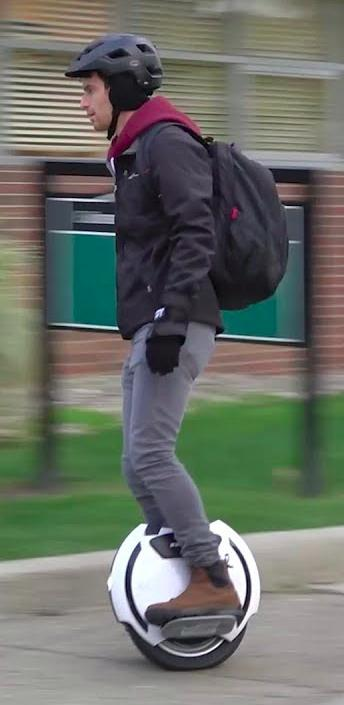
\includegraphics[width=0.6\textwidth]{images/unicycle_2.jpg}}
        \end{column}
        \begin{column}[c]{0.6\textwidth}
            \centering
            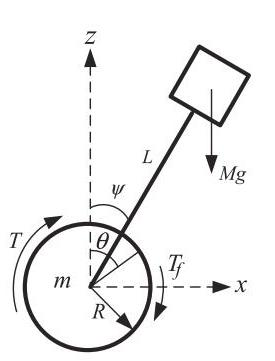
\includegraphics[width=.6\textwidth]{images/unicycle_model.jpg}
        \end{column}
    \end{columns}   
\end{frame}



\begin{frame}[t]{Referências}
    \begin{itemize}
        \item Craig, John J. "Robótica. 3ª edição." Rev. Atual (2012).      
    \end{itemize}
\end{frame}
\end{document}